\subsection{Integral-Gesetze der Elektrotechnik}
	
	\begin{tabular}{|p{2.5cm}||p{2.7cm}|p{4cm}|p{2.7cm}|p{5cm}|}
	\hline
	& \textbf{Elektr. Feld} & \textbf{Magn. Feld} & \textbf{Strömungsfeld} & 		
			\textbf{Bemerkung}\\
	\hline \hline
	Feldgrösse & $\vec{E}$, $\vec{D}$ & $\vec{H}$, $\vec{B}$
		& $\vec{E}$, $\vec{J}$ &\\
	\hline
	Konstante
		& \parbox{2.7cm}{$\varepsilon_0 = 8.854 \cdot 10^{-12}$\\
		{\tiny Dielektrizitätskonstante} \vspace{.1cm}} 
		& \parbox{4cm}{$\mu_0 = 4 \pi \, 10^{-7}$\\ {\tiny Permeabilitätskonstante} \vspace{.1cm}} 
		& \parbox{2.7cm}{$\sigma=\frac{1}{\rho}$ \\ {\tiny Spezifische
		Leitfähigkeit}\vspace{.1cm}} &\\ 
	\hline
	Stoffgleichung & $\vec{D}=\varepsilon_0\varepsilon_r\vec{E}$ & 	
		$\vec{B}=\mu_0\mu_r\vec{H}$
	& $\vec{J}=\sigma\vec{E}$ &
	\\
	\hline
	Kraft & $\vec{F_C}=q\vec{E}$ & $\vec{F_L}=q(\vec{v}\times\vec{B})$ &&\\
	\hline
	\parbox{2.5cm}{Fluss\\{\tiny (durch Fläche A)}} & $\Psi_{el}=\int\vec{D}\vec{dA}$ &
	$\Phi_m=\int\vec{B}\vec{dA}$ \textsuperscript{1)}&
	$I=\int\vec{J}\vec{dA}$ & \textsuperscript{1)} bei Spulen:
	$\Psi_m=\sum_i\Phi_i\approx N \Phi$\\
	\hline
	\parbox{2.5cm}{Spannung \\{\tiny (Weg A$\to$B)}} & $U_{AB}=\int\limits_{A}^B
	\vec{E}\vec{ds}$ & $V_{m_{AB}}=\int\limits_{A}^B\vec{H}\vec{ds} = \Theta$ 
	& $U_{AB}=\int\limits_{A}^B\vec{E}\vec{ds}$ & \\
	\hline
	Schaltelemente & $Q=CU$ & $\Psi_m=LI$, $\Psi_{m21}=M_{21}I_1$
	& $I=GU$, $U=RI$ & $R_m=\frac{1}{\Lambda}$, $R=\frac{1}{G}$\\
	\hline
	\parbox{2.5cm}{Hüllengesetz \\ {\tiny (Quellengleichungen)}}
		& \parbox{2.7cm}{
			\vspace{.1cm}$\oint\vec{D}\vec{dA}=\sum Q_i$ \vspace{.1cm}
			Maxwell IV
			\vspace{.1cm}}
		& \parbox{4cm}{
			\vspace{.1cm}$\oint\vec{B}\vec{dA}=0$
			\textsuperscript{2)} \\
			Maxwell III
			\vspace{.1cm}} 
		& \parbox{2.7cm}{
			$\oint\vec{J}\vec{dA}=0$\\
			Kirchhoff 1}
		& \parbox{5cm}{\textsuperscript{2)} ohne Verschiebungsstrom (käme ggf. noch
		dazu)} \\
	\hline
	Umlaufspannung 
		& \parbox{2.7cm}{
			\vspace{.1cm}
			$\oint\vec{E}\vec{ds}=0-\dot{\Phi}_m$ \\ 
			{\tiny Induktionsgesetz}\\Maxwell II
			\vspace{.1cm}}
		& \parbox{4cm}{
			\vspace{.1cm}
			$\oint\vec{H}\vec{ds}=\theta+\dot{\Psi}_{el}$ \\ 
			{\tiny Vollständiges Durchflutungsgesetz} \\Maxwell I
			\vspace{.1cm}}
		& \parbox{2.7cm}{
			\vspace{.1cm}
			$\oint\vec{E}\vec{ds}=0-\dot{\Phi}$ \\ Kirchhoff 2
			\vspace{.1cm}}
		& \\
	\hline
	\end{tabular}
	
	
\subsection{Einheiten}

	\begin{tabular}{|l|l|l|l|l|l|}
	\hline
	$[\varepsilon] = \frac{As}{Vm}$
		& $[D] = \frac{As}{m^2} = \frac{C}{m^2}$
		& $[E] = \frac{V}{m}$
		& $[U] = V$
		& $[\Psi_{el}] = As = C$
		& $[C] = F$ \\
	\hline
	$[\mu] = \frac{H}{m}=\frac{V s}{A m}$
		& $[B] = \frac{Vs}{m^2} = T$
		& $[H] = \frac{A}{m}$
		& $[V_m] = [\Theta] = A$
		& $[\Psi_m] = [\Phi_m] = Wb = Vs$
		& $[L] = \frac{Vs}{A} = H$ \\
	\hline
	$[\sigma] = \frac{S}{m}$
		& $[E] = \frac{V}{m}$
		& $[J] = \frac{A}{m^2} = 10^{-6} \frac{A}{mm^2}$
		& $[U] = V$
		& $[I] = A$
		& $[R] = \Omega$ \\
	\hline
	\end{tabular}
	

\subsection{Magnetismus}

Magnetische Feldlinien verlaufen ausserhalb eines Magneten vom Nord- zum Südpol
und sind immer geschlossen.\\ 
	
	\begin{tabular}[c]{ | p{5cm} | p{8.7cm} | p{4cm} | }
		\hline
		\textbf{Name} & \textbf{Formel} & \textbf{Bemerkung}\\    
		\hline
		\hline
		Lorentzkraft
		& $\vec{F} = Q (\vec{v} \times \vec{B})=I(\vec{l}\times \vec{B}) \hspace{1cm} |\vec{F}| = Q \cdot v \cdot B
		\cdot \sin\alpha$
		&$[\vec{F}]= N$\\
		\hline
		Rechte-Hand-Regel
		& $F$ = Daumen; $v$, $I$ = Zeigefinger; $B$ = Mittelfinger
		& Bei $Q < 0$ wechselt Richtung von B!\\
		\hline
		\parbox{5cm}{Induktionsgesetz\\ \tiny{Allgemeine Form}} &
		$u_i= \mp \dot{\Phi} = \mp \frac{d}{dt} \int \vec{B} \cdot
		\vec{dA}\qquad $ \parbox{3cm}{\tiny{$- \Rightarrow B,u_i $
		Rechtsschraube\\ $+ \Rightarrow B,u_i $
		Linksschraube}} & $[u_i]= V$\\
		& $u_i= \mp \dot{\Psi}\qquad$ , meist $\; u_i = \mp
		N\cdot\dot{\Phi}$ &
		\\
		\hline
		\parbox{5cm}{Induktionsgesetz\\ \tiny{bewegter Leiter im Magnetfeld}} &
		$u_i=\int\vec{E}_i \cdot
		\vec{dl}=-\int(\vec{v}\times \vec{B})\cdot\vec{dl}$ & $[u_i]= V$\\
		& $u_i=v\cdot B \cdot l\qquad$ falls $\vec{v}\perp \vec{B}$ &\\	

		\hline		
		Durchflutungsgesetz
		& $V_m = \oint\vec{H} \cdot \vec{ds} = \int\limits \vec{J}
		\cdot \vec{dA} \vee \underbrace{\sum I_k}_{= N I} = \Theta$
		& $[V_m,\Theta]=A$\\
		\hline
		Magn. Widerstand / Leitwert
		& $R_m = \frac{V_m}{\Phi} = \frac{\Theta}{\Phi} = \frac{l}{\mu A} $ \quad / \quad
		$\Lambda = \frac{1}{R_m}$ & $[R_m]=\frac{A}{Wb}$\;
		/ \;$[\Lambda]=\frac{Wb}{A}$
		\\
		\hline
		Induktivität
		& $L = \frac{\Psi}{I}  \qquad \text{Bei idealer Koppl.: } L = \Lambda N^2 = \frac{N^2}{R_m} $
		& $[L] = \frac{Vs}{A} = H$\\
		\hline
	\end{tabular}
	


\subsection{Zusammenstellung magnetischer Grössen für spezielle
Leiteranordnungen}
\begin{tabular}{|p{5cm}|l|l|l|l|l|}
  \hline
  & Leitwert $ \Lambda $ & Durchfl. $ \Theta $ & Fluss $ \Phi ^{1)} $ &
  Verk.-Fluss $ \Psi $ & Induktivität $L^{2)}$ \\
  \hline
  Kreisförmige Schleife & $\frac{\mu D}{2}\cdot\ln\frac{D}{d}$ & $\Theta = I$ & $\frac{\mu D}{2}\cdot\ln\frac{D}{d}\cdot I$ & $\Psi = \Phi$ & $L=\frac{\mu
  D}{2}\cdot\ln\frac{D}{d}$\\
  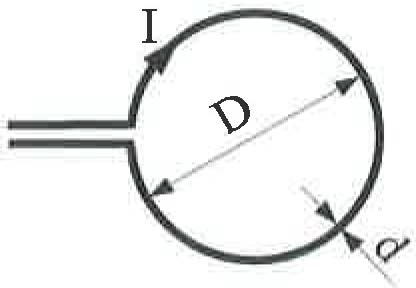
\includegraphics[width=2.5cm]{./images/kreisfoermige_schleife.png} & & & & & \\
  \hline
  Kreisrahmenspule$^{3)}$ & $\frac{\mu D}{2}\cdot\ln\frac{D}{d}$ & $\Theta = NI$ & $\frac{\mu D}{2}\cdot\ln\frac{D}{d}\cdot N \cdot I$ & $\Psi = N \cdot \Phi$ & $L=\frac{\mu  D}{2}\cdot\ln\frac{D}{d}\cdot N^2$\\
  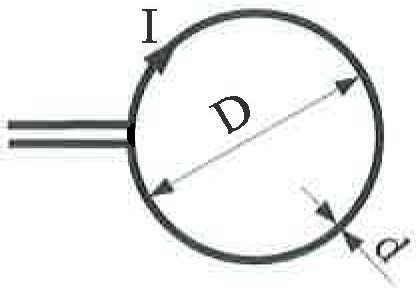
\includegraphics[width=2.5cm]{./images/kreisrahmenspule.png} & & & & & \\
  \hline
  Zylinderspule $l \gg d$
  & $\frac{\mu A}{l} = \frac{\mu \pi d^2}{4l}$ & $\Theta = NI$ & $\frac{\mu \pi d^2}{4l} \cdot N \cdot I$ & $\Psi = N \cdot \Phi$ & $L=\frac{\mu \pi d^2}{4l}\cdot N^2$\\
  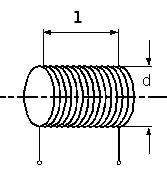
\includegraphics[width=2.5cm]{./images/zylinderspule.png} & & & & & \\
  \hline
  Toroidspule $^{4)}$ & $\frac{\mu A}{l_m} = \frac{\mu d^2}{4 D_m}$ & $\Theta = NI$ & $\frac{\mu d^2}{4 D_m}\cdot N \cdot I$ & $\Psi = N
  \cdot \Phi$ & $L=\frac{\mu d^2}{4 D_m}\cdot
  N^2$\\
  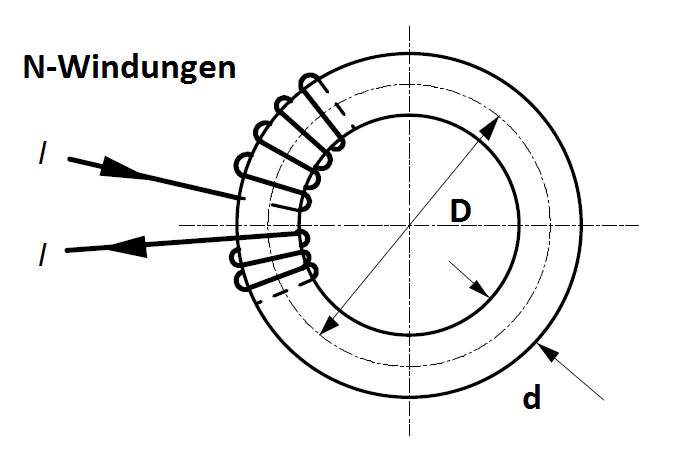
\includegraphics[width=3.5cm]{./images/toroidspule.png} & & & & & \\
  \hline
  Ringspule mit rechteckf. Querschnitt & $\frac{\mu a}{2
  \pi}\cdot\ln\frac{D}{d}$ & $\Theta = NI$ & $\frac{\mu a}{2\pi}\cdot\ln\frac{D}{d}\cdot N \cdot I$ & $\Psi = N
  \cdot \Phi$ & $L=\frac{\mu a}{2\pi}\cdot\ln\frac{D}{d}\cdot N^2$\\
  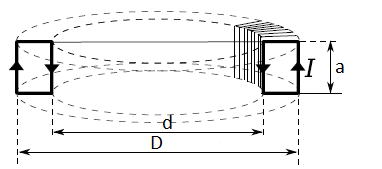
\includegraphics[width=4cm]{./images/torus.png} & & & & & \\
  \hline
  Koaxialleitung $R_2 > R_1$
  & $\frac{\mu l}{2 \pi}\cdot\ln\frac{R_2}{R_1}$ & $\Theta = I$ & $\frac{\mu l}{2\pi}\cdot\ln\frac{R_2}{R_1}\cdot I$ & $\Psi = \Phi$ & $L=\frac{\mu l}{2\pi}\cdot\ln\frac{R_2}{R_1}$ \\
  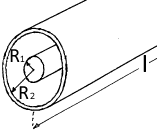
\includegraphics[width=2.5cm]{./images/e-c-koaxialkabel.png} & & & & & \\
  \hline
  Paralleldrahtleitung $l \gg a \gg R$ & $\frac{\mu l}{\pi}\cdot\ln\frac{a-R}{R}$ & $\Theta = I$ & $\frac{\mu l}{\pi}\cdot\ln\frac{a-R}{R}\cdot I$ & $\Psi = \Phi$ & $L=\frac{\mu l}{\pi}\cdot\ln\frac{a-R}{R}$\\
  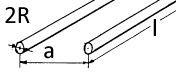
\includegraphics[width=2.5cm]{./images/e-c-paralleldraht.png} & & & & & \\
  \hline
\end{tabular}

\begin{multicols}{2}
	\textbf{Bemerkungen:}\\
	$^{1)}$ ohne Fluss durch Leiter\\
	$^{2)}$ nur äussere Induktivität\\
	$^{3)}$ Wicklungs-$\varnothing$ d in radialer und axialer Richtung $d \ll D$\\
	$^{4)}$ $A=\frac{\pi d^2}{4} \qquad l_m \approx \pi D_m$\\
	
	\textbf{Allgemein} gilt:\\
	$\Phi=\Lambda \cdot \Theta$, $\Lambda=\frac{1}{R_m}$\\
	$L=\frac{\Psi}{I}$\\
	$L=\Lambda=\frac{1}{R_m}$, falls $N=1$\\
	$L=\Lambda N^2=\frac{N^2}{R_m}$, falls die $N$-Windungen\\ unter sich ideal
	gekoppelt sind.
\end{multicols}

\subsection{Diverse Formeln bzgl. Magnetismus}

\begin{tabular}[c]{|l|l|l|}
\hline
M'feld ausserhalb langen Leiters:
	& M'feld innerhalb geraden, langen Leiters: 
	& Hall-Sonde:\\
$H(r) = \frac{I}{2 \cdot \pi \cdot r}$
	&$H(r) = \frac{I}{2 \pi r} \frac{A_{eingeschlossen}}{A_{total}} = 
	 \frac{I}{2 \pi} \frac{r}{r_a^2}$
	& $U_H = \frac{I \cdot B}{e \cdot n_p \cdot h}$\\
\hline
M'feld der Zylinderspule:
	&M'feld einer Toroidspule:
	&Kraft auf stromführende Leiter:\\
$H(r) = \frac{N \cdot I}{l} \qquad l \gg d$
	& $H_{innen}(r) = \frac{N \cdot I}{2 \cdot \pi \cdot r} \qquad H_{aussen} = 0$
	&$\vec{F_L} = I (\vec{l} \times \vec{B}) \qquad F_L = I \cdot l \cdot B \cdot
	\sin{\alpha}$ \\
\hline
\end{tabular}\\


\begin{tabular}{llll}
\parbox{4.5cm}{
	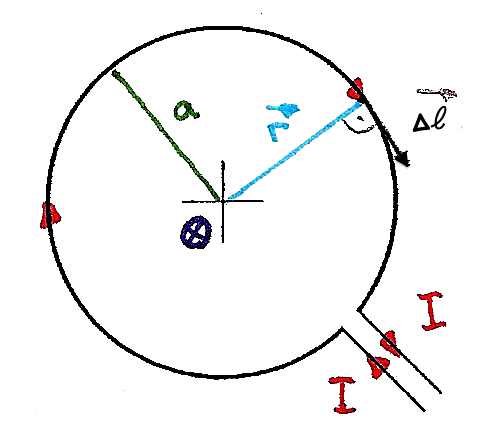
\includegraphics[width=2.7cm]{./images/biot1.png} \\
	$H =\frac{I}{D} = \frac{I}{2a}$}
& \parbox{4.5cm}{
	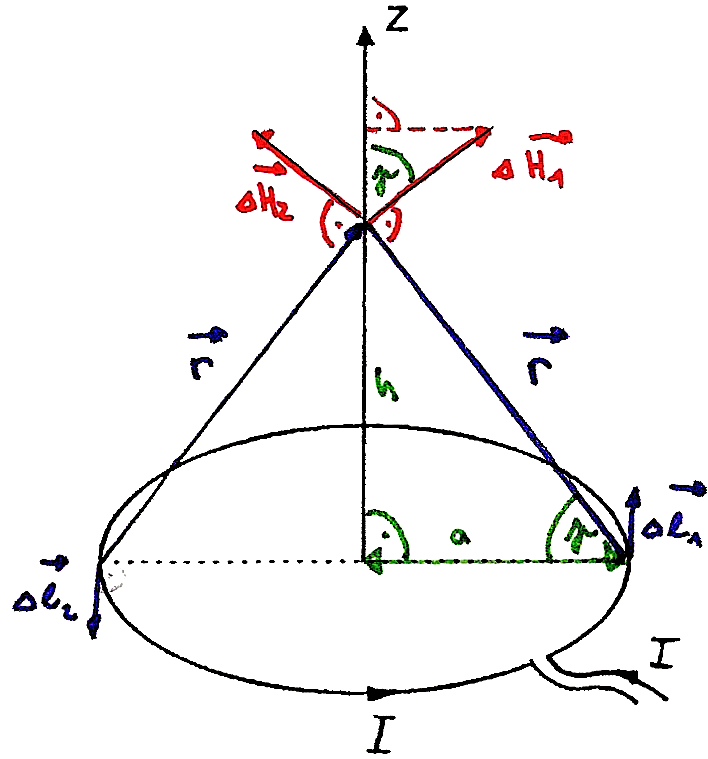
\includegraphics[width=2.7cm]{./images/biot2.png} \\
	$H=\frac{I}{2} \cdot \frac{a^2}{\sqrt{a^2+h^2}^3}$}
& \parbox{4.5cm}{
	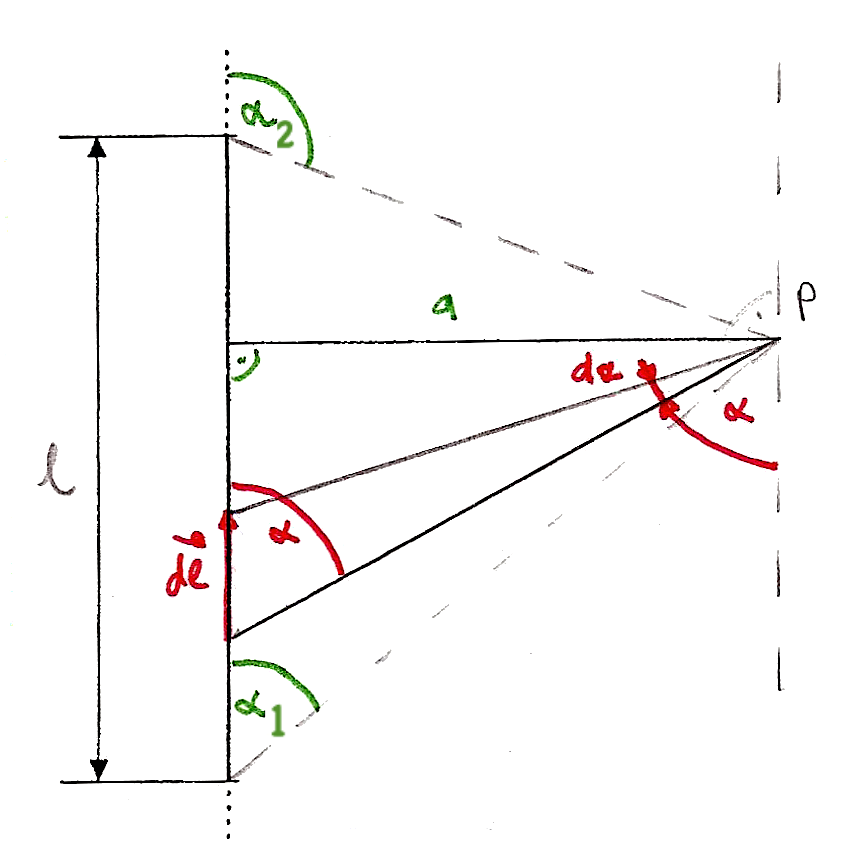
\includegraphics[width=3cm]{./images/biot3.png} \\
	$H=\frac{I}{4\pi a}(\cos(\alpha_1)- \cos(\alpha_2))$}
& \parbox{4.5cm}{
	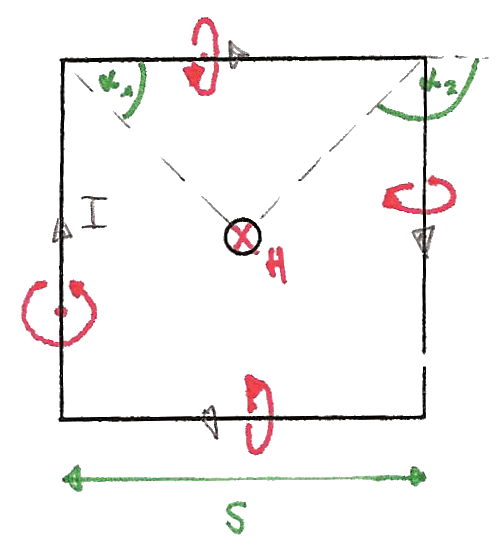
\includegraphics[width=2.7cm]{./images/biot4.png} \\
	$H= \frac{I \cdot 2 \sqrt{2}}{\pi \cdot s}$ }
\end{tabular}

\subsection{Gegeninduktion, Transformator}
\definecolor{red}{rgb}{1,0,0} % 255,0,0
\definecolor{green}{rgb}{0,.8,0.05} % 0,203,14
\begin{tabular}{ll}
	\parbox{9.5cm}{
 		\textbf{Gegeninduktion} ($M_{\textcolor{red}{X}\textcolor{green}{Y}}; \textcolor{red}{X}$: Wirkung,
 		$\textcolor{green}{Y}$: Ursache)\\
		\begin{tabular}{ll}
  		Gegeninduktivität
  			& $M_{21} = \frac{\Psi_{m21}}{i_1} =$ (Meist $= \frac{N_2
  			\phi_{m21}}{i_1}$)\\ 
  			(wenn $\mu$ = const.) & $M = k \cdot \sqrt{L_1 L_2} = M_{21} = M_{12} $  \\
  			Gegeninduktionsspannung
  			& $u_{21} = \dot{\Psi}_{21} = M_{21} \frac{di_1}{dt}$    
		\end{tabular}}
	& \parbox{8.5cm}{
	  	Durchsetzt das sich ändernde Magnetfeld einer stromdurchflossenen Spule
	  	eine zweite Spule, so wird auch in dieser eine Spannung
	  	(=Gegeninduktionsspannung) induziert.}\\
\parbox{9.5cm}{
		\vspace{.2cm}
  		\textbf{Transformatorgleichungen}\\
		\fbox{$u_1 = L_1 \dfrac{di_1}{dt} \textcolor{red}{+}\textcolor{green}{-}M_{12} \dfrac{di_2}{dt} 
			= L_1 \dfrac{di_1}{dt} \textcolor{red}{-}\textcolor{green}{+}M_{12} \dfrac{di_b}{dt}$} $\qquad$ 
		\fbox{$u_2 = L_2 \dfrac{di_2}{dt}
		\textcolor{red}{+}\textcolor{green}{-} M_{21} \dfrac{d i_1}{dt} 
			= -L_2 \dfrac{di_b}{dt} \textcolor{red}{+}\textcolor{green}{-} M_{21}
			\dfrac{d i_1}{dt}$} 
		\vspace{.2cm}
  			
	  		\textbf{Idealer Trafo}\\ 
	  		\fbox{$"u = \dfrac{u_1}{u_2} = \dfrac{N_1}{N_2} = n$} $\qquad$ (im Leerlauf: $\dfrac{1}{"u} = k \sqrt{\dfrac{L_2}{L_1}}$)
	  		}
  		& \parbox{5cm}{
	  		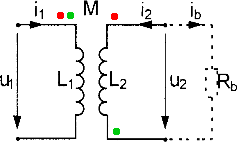
\includegraphics[width=4cm]{./images/trafo-kopplung.png} \\
      		\small{\textcolor{red}{Gleichsinnig} / \textcolor{green}{Gegensinnig}}} \\
	  		
  	\parbox{9.7cm}{
      		\textbf{Verlustbehafteter Trafo}
      		\begin{list}{$\bullet$}{\setlength{\itemsep}{0cm} \setlength{\parsep}{0cm} \setlength{\topsep}{0cm}} 
              \item Primärstrom im Leerlauf: $L_H$
	          	(ideal $L_H \rightarrow \infty)$
	          \item Hysterese- \& Wirbelstromverluste: $R_{Fe}$
	          	(ideal: $R_{Fe}
	          \rightarrow \infty$) 
	          \item Kupferwiderstände: $R_{Cu1}, R_{Cu2}$
	          	(ideal: $R_{Cu}
	          \rightarrow 0$)
	          \item Streufluss (Kopplung): $L_{\sigma1}, L_{\sigma2}$
	          	(ideal: $L_{\sigma} \rightarrow 0$)
            \end{list}
      		}
  		& \parbox{8.8cm}{
	  		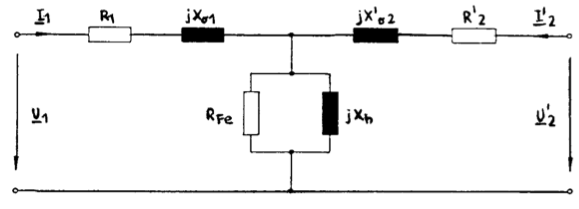
\includegraphics[width=8.8cm]{./images/trafo-verluste.png}}
   	\end{tabular}